% LaTeX support: latex@mdpi.com 
% In case you need support, please attach all files that are necessary for compiling as well as the log file, and specify the details of your LaTeX setup (which operating system and LaTeX version / tools you are using).

% You need to save the "mdpi.cls" and "mdpi.bst" files into the same folder as this template file.

%=================================================================
\documentclass[ijgi,article,submit,moreauthors,pdftex,10pt,a4paper]{Definitions/mdpi} 
\usepackage{subfig, amsmath, amsfonts}

% If you would like to post an early version of this manuscript as a preprint, you may use preprint as the journal and change 'submit' to 'accept'. The document class line would be, e.g. \documentclass[preprints,article,accept,moreauthors,pdftex,10pt,a4paper]{mdpi}. This is especially recommended for submission to arXiv, where line numbers should be removed before posting. For preprints.org, the editorial staff will make this change immediately prior to posting.

%
%--------------------
% Class Options:
%--------------------
% journal
%----------
% Choose between the following MDPI journals:
% acoustics, actuators, addictions, admsci, aerospace, agriculture, agronomy, algorithms, animals, antibiotics, antibodies, antioxidants, applsci, arts, asi, atmosphere, atoms, axioms, batteries, bdcc, behavsci, beverages, bioengineering, biology, biomedicines, biomimetics, biomolecules, biosensors, brainsci, buildings, carbon, cancers, catalysts, cells, ceramics, challenges, chemengineering, chemosensors, children, cleantechnol, climate, clockssleep, cmd, coatings, colloids, computation, computers, condensedmatter, cosmetics, cryptography, crystals, cybersecurity, data, dentistry, designs, diagnostics, dairy, diseases, diversity, drones, econometrics, economies, education, electrochem, electrochemistry, electronics, energies, entropy, environments, epigenomes, est, fermentation, fibers, fire, fishes, fluids, foods, forecasting, forests, fractalfract, futureinternet, galaxies, games, gastrointestdisord, gels, genealogy, genes, geohazards, geosciences, geriatrics, hazardousmatters, healthcare, heritage, highthroughput, horticulturae, humanities, hydrology, informatics, information, infrastructures, inorganics, insects, instruments, ijerph, ijfs, ijms, ijgi, ijtpp, inventions, j, jcdd, jcm, jcs, jdb, jfb, jfmk, jimaging, jof, jintelligence, jlpea, jmmp, jmse, jpm, jrfm, jsan, land, languages, laws, life, literature, logistics, lubricants, machines, magnetochemistry, make, marinedrugs, materials, mathematics, mca, medsci, medicina, medicines, membranes, metabolites, metals, microarrays, micromachines, microorganisms, minerals, modelling, molbank, molecules, mps, mti, nanomaterials, ncrna, neonatalscreening, neuroglia, nitrogen, nutrients, ohbm, particles, pathogens, pharmaceuticals, pharmaceutics, pharmacy, philosophies, photonics, plants, plasma, polymers, polysaccharides, proceedings, processes, proteomes, publications, quaternary, qubs, reactions, recycling, religions, remotesensing, reports, resources, risks, robotics, safety, sci, scipharm, sensors, separations, sexes, sinusitis, smartcities, socsci, societies, soilsystems, sports, standards, stats, surfaces, surgeries, sustainability, symmetry, systems, technologies, toxics, toxins, tropicalmed, universe, urbansci, vaccines, vehicles, vetsci, vibration, viruses, vision, water, wem, wevj
%---------
% article
%---------
% The default type of manuscript is article, but can be replaced by: 
% abstract, addendum, article, benchmark, book, bookreview, briefreport, casereport, changes, comment, commentary, communication, conceptpaper, correction, conferenceproceedings, conferencereport, expressionofconcern, meetingreport, creative, datadescriptor, discussion, editorial, essay, erratum, hypothesis, interestingimages, letter, meetingreport, newbookreceived, opinion, obituary, projectreport, reply, reprint, retraction, review, perspective, protocol, shortnote, supfile, technicalnote, viewpoint
% supfile = supplementary materials
% protocol: If you are preparing a "Protocol" paper, please refer to http://www.mdpi.com/journal/mps/instructions for details on its expected structure and content.
%----------
% submit
%----------
% The class option "submit" will be changed to "accept" by the Editorial Office when the paper is accepted. This will only make changes to the frontpage (e.g. the logo of the journal will get visible), the headings, and the copyright information. Also, line numbering will be removed. Journal info and pagination for accepted papers will also be assigned by the Editorial Office.
%------------------
% moreauthors
%------------------
% If there is only one author the class option oneauthor should be used. Otherwise use the class option moreauthors.
%---------
% pdftex
%---------
% The option pdftex is for use with pdfLaTeX. If eps figures are used, remove the option pdftex and use LaTeX and dvi2pdf.

%=================================================================
\usepackage{amsmath}
\usepackage{amsfonts}
\def\A{{\mathbf A}}
\def\U{{\mathbf U}}
\def\V{{\mathbf V}}
\def\S{{\mathbf S}}
\def\u{{\mathbf u}}
\def\v{{\mathbf v}}
\def\s{{\mathbf s}}
\firstpage{1} 
\makeatletter 
\setcounter{page}{\@firstpage} 
\makeatother
\pubvolume{xx}
\issuenum{1}
\articlenumber{1}
\pubyear{2018}
\copyrightyear{2018}
\externaleditor{Academic Editor: name}
\history{Received: date; Accepted: date; Published: date}
%\updates{yes} % If there is an update available, un-comment this line

%------------------------------------------------------------------
% The following line should be uncommented if the LaTeX file is uploaded to arXiv.org
%\pdfoutput=1

%=================================================================
% Add packages and commands here. The following packages are loaded in our class file: fontenc, calc, indentfirst, fancyhdr, graphicx, lastpage, ifthen, lineno, float, amsmath, setspace, enumitem, mathpazo, booktabs, titlesec, etoolbox, amsthm, hyphenat, natbib, hyperref, footmisc, geometry, caption, url, mdframed, tabto, soul, multirow, microtype, tikz

%=================================================================
%% Please use the following mathematics environments: Theorem, Lemma, Corollary, Proposition, Characterization, Property, Problem, Example, ExamplesandDefinitions, Hypothesis, Remark, Definition
%% For proofs, please use the proof environment (the amsthm package is loaded by the MDPI class).

%=================================================================
% Full title of the paper (Capitalized)
\Title{Dataset Reduction Techniques to Speed Up SVD Analyses on Big Geo-DataSets}

% Author Orchid ID: enter ID or remove command
\newcommand{\orcidauthorA}{0000-0002-7712-6627} % Add \orcidA{} behind the author's name
\newcommand{\orcidauthorB}{0000-0003-2225-1428} % Add \orcidB{} behind the author's name
\newcommand{\orcidauthorC}{0000-0002-1769-6310} % Add \orcidC{} behind the author's name
\newcommand{\orcidauthorD}{0000-0003-2179-1262} % Add \orcidC{} behind the author's name

% Authors, for the paper (add full first names)

\Author{Laurens Bogaardt $^{1}$\orcidA{}, Romulo Goncalves $^{1}$\orcidB{}, Raul Zurita-Milla $^{2,}$*\orcidC{} and Emma Izquierdo-Verdiguier $^{3}$\orcidD{}}

% Authors, for metadata in PDF
\AuthorNames{Laurens Bogaardt, Romulo Goncalves, Raul Zurita-Milla, Emma Izquierdo-Verdiguier}

% Affiliations / Addresses (Add [1] after \address if there is only one affiliation.)
\address{%
$^{1}$ \quad Netherlands eScience Center; l.bogaardt@esciencecenter.nl, r.goncalves@esciencecenter.nl\\
$^{2}$ \quad Faculty ITC, University of Twente; r.zurita-milla@utwente.nl\\
$^{3}$ \quad IVFL, University of Natural Resources and Life Sciences (BOKU); emma.izquierdo@boku.ac.at}

% Contact information of the corresponding author
\corres{Correspondence: r.zurita-milla@utwente.nl}

% Current address and/or shared authorship
%\firstnote{Current address: Affiliation 3} 
%\secondnote{These authors contributed equally to this work.}
% The commands \thirdnote{} till \eighthnote{} are available for further notes

% Simple summary
%\simplesumm{}

%\conference{} % An extended version of a conference paper

% Abstract (Do not insert blank lines, i.e. \\) 
\abstract{The Singular Value Decomposition (SVD) is a mathematical procedure with multiple applications in the geosciences. For instance, it is used in
dimensionality reduction and as a support operator for various analytical tasks applicable to spatio-temporal data. Performing SVD analyses on large
datasets, however, can be computationally costly, time consuming and sometimes practically infeasible. Yet, techniques exist to arrive at the same
output, or at a close approximation, which require far less effort. This article examines several such techniques in relation to the inherent scale of
the structure within the data. When the values of a dataset vary slowly, e.g. in a spatial field of temperature over a country, there is autocorrelation and the field contains large scale structure. Datasets do not need a high resolution to describe such fields and their analysis can benefit from
alternative SVD techniques based on rank deficiency, coarsening or matrix factorization approaches. We use both simulated Gaussian Random Fields
with various levels of autocorrelation and real-world geospatial datasets to illustrate our study while examining the accuracy of various SVD
techniques. As the main result, this article provides researchers with a decision tree indicating which technique to use when and predicting the
resulting level of accuracy based on the dataset's structure scale.}

%We use both simulated Gaussian Random Fields with various levels of autocorrelation and real-world geospatial datasets to illustrate our study while examining the accuracy or correctness of various SVD techniques. Our experimental results link the autocorrelation level in geo-datasets with the singular values of the data matrix and can guide researchers regarding which SVD technique to use when.}

% Keywords
\keyword{Singular value decomposition, autocorrelation, rank deficiency, data reduction, coarsening, approximate SVD, Gaussian Random Fields}

% The fields PACS, MSC, and JEL may be left empty or commented out if not applicable
%\PACS{J0101}
%\MSC{}
%\JEL{}

%%%%%%%%%%%%%%%%%%%%%%%%%%%%%%%%%%%%%%%%%%
% Only for the journal Applied Sciences:
%\featuredapplication{Authors are encouraged to provide a concise description of the specific application or a potential application of the work. This section is not mandatory.}
%%%%%%%%%%%%%%%%%%%%%%%%%%%%%%%%%%%%%%%%%%

%%%%%%%%%%%%%%%%%%%%%%%%%%%%%%%%%%%%%%%%%%
% Only for the journal Data:
%\dataset{DOI number or link to the deposited data set in cases where the data set is published or set to be published separately. If the data set is submitted and will be published as a supplement to this paper in the journal Data, this field will be filled by the editors of the journal. In this case, please make sure to submit the data set as a supplement when entering your manuscript into our manuscript editorial system.}

%\datasetlicense{license under which the data set is made available (CC0, CC-BY, CC-BY-SA, CC-BY-NC, etc.)}

%%%%%%%%%%%%%%%%%%%%%%%%%%%%%%%%%%%%%%%%%%
% Only for the journal Toxins
%\keycontribution{The breakthroughs or highlights of the manuscript. Authors can write one or two sentences to describe the most important part of the paper.}

%\setcounter{secnumdepth}{4}
%%%%%%%%%%%%%%%%%%%%%%%%%%%%%%%%%%%%%%%%%%
\begin{document}
%%%%%%%%%%%%%%%%%%%%%%%%%%%%%%%%%%%%%%%%%%
%% Only for the journal Gels: Please place the Experimental Section after the Conclusions

%%%%%%%%%%%%%%%%%%%%%%%%%%%%%%%%%%%%%%%%%%
%\setcounter{section}{-1} %% Remove this when starting to work on the template.
%\section{How to Use this Template}
%The template details the sections that can be used in a manuscript. Note that the order and names of article sections may differ from the requirements of the journal (e.g. the positioning of the Materials and Methods section). Please check the instructions for authors page of the journal to verify the correct order and names. For any questions, please contact the editorial office of the journal or support@mdpi.com. For LaTeX related questions please contact Janine Daum at latex-support@mdpi.com.
%The order of the section titles is: Introduction, Materials and Methods, Results, Discussion, Conclusions for these journals: aerospace,algorithms,antibodies,antioxidants,atmosphere,axioms,biomedicines,carbon,crystals,designs,diagnostics,environments,fermentation,fluids,forests,fractalfract,informatics,information,inventions,jfmk,jrfm,lubricants,neonatalscreening,neuroglia,particles,pharmaceutics,polymers,processes,technologies,viruses,vision

\section{Introduction} % RG and LB: put focus on Out-of-core?
\label{sec:Introduction} % RZ: I miss a bit of literature review. what have others (particularly in the domain of geosciences) done with SVDs? or to study autocorrelation? 

%The introduction should briefly place the study in a broad context and highlight why it is important. It should define the purpose of the work and its significance. The current state of the research field should be reviewed carefully and key publications cited. Please highlight controversial and diverging hypotheses when necessary. Finally, briefly mention the main aim of the work and highlight the principal conclusions. As far as possible, please keep the introduction comprehensible to scientists outside your particular field of research. Citing a journal paper \cite{ref-journal}. And now citing a book reference \cite{ref-book}. Please use the command \citep{ref-journal} for the following MDPI journals, which use author-date citation: Administrative Sciences, Arts, Econometrics, Economies, Genealogy, Humanities, IJFS, JRFM, Languages, Laws, Religions, Risks, Social Sciences.

The \textit{Singular Value Decomposition} (SVD) is a linear algebra procedure used to factorize a matrix $\A$ as a product of three matrices, $\U$,$\V$,
and $\S$, where the matrices $\U$ and $\V$ are orthonormal and $\S$ is a diagonal matrix that contains the so-called singular values~\cite{Golub1970}.
This matrix decomposition has found multiple applications in both engineering and scientific disciplines \cite{Rajwade13, khoshbin16, meuwissen17}. In
the geosciences, SVD helps to identify structure when analysing a spatial field for a single time period. In many real-world applications, however,
spatial fields include multiple time periods or contain multiple thematic attributes such as spectral bands. In these cases, an SVD can
help to eliminate some of the redundancy between time periods or attributes as well as between neighbouring locations (pixels in images and grid cells
in rasters). The SVD can thus be seen as an efficient dimensionality reduction technique which facilitates further analysis. For instance, the SVD
helps to obtain accurate products of spatio-temporal fields (matrices), and to reduce the deficiencies of the acquired data (noise or non-linear
nature)~\cite{izquierdo17}. Moreover, several analytical approaches commonly used in the geosciences are based on the SVD, such as the \textit{Partial Least Squares} (PLS) method in classification and regression tasks and the \textit{Maximum Covariance Analysis}
(MCA) and \textit{Canonical Correlation Analysis} (CCA) methods, which are often used to analyse multi-temporal datasets~\cite{izquierdo14, hansen03, munoz13}. A combination of CCA with \textit{Minimum Noise Fraction} (MNF) has proven successful at filtering out noise from
images~\cite{nielsen07}. Last but not least, the SVD has been used to compare ground data and measurements done by Earth observation
satellites~\cite{li14, li14b}. This is because SVD offers an effective method to find frequent and simultaneous patterns between two spatio-temporal
fields~\cite{Eshel2011, Storch1999}.

Performing SVD's on large datasets can be computationally costly and time consuming. This is especially true when the datasets themselves are too
large to fit in \textit{RAM}-memory, or when an intermediate step in the analysis becomes excessively large. Often, techniques exist to arrive at the
same output, or at a close approximation, which require far less effort. This article examines several SVD procedures which exploit autocorrelation
and rank decomposition to analyse data in an efficient manner. We explain which type of problems could be tackled with them and make predictions about
the error incurred in the approximations based on the level of autocorrelation of the input data. Though the individual techniques are not novel, to
the best of our knowledge, this is the first review in the geosciences which examines SVD implementations for big geo-datasets from the point of view of
autocorrelation and data reduction~\cite{Golub1970, Bjorck1973, Chan1982}.

To arrive at these results, we will simulate geo-datasets with various levels of autocorrelation and subsequently reduce them in size. The amount of error
incurred in this reduction is determined by comparing the SVD of the reduced dataset to that of the original. Finally, the techniques and predictions,
based on simulated data, are verified using real-world geospatial datasets. The reported results come from calculations performed in an accompanying
\textit{Jupyter Notebook}, which can be found in the online supplementary material~\cite{Bogaardt2018}.

The paper is outlined as follows. Section~\ref{sec:Materials and Methods} reviews some matrix algebra and describes the concept of autocorrelation. Section~\ref{sec:Results} explains the different SVD implementations and presents the the simulated and real-world data sets used in their study
as well as our experimental results. Finally,~section \ref{sec:Discussion} summarizes our main findings and recommendations.

\section{Materials and Methods}
\label{sec:Materials and Methods}

This section reviews some matrix algebra and expands on a method to simulate fields which resemble those often encountered in real-world
applications. Additionally, we discuss how to measure the level of autocorrelation of a~field.

\subsection{Matrix Decomposition}
\label{sec:Materials and Methods/Matrix Decomposition}

Many geo-datasets can be represented as a matrix.
For instance, temperatures measured at~$m$ locations for~$n$ time periods can be arranged in a matrix with~$m$ rows and~$n$ columns. From a linear
algebra perspective, this matrix is nothing more than a linear combination of basis vectors that indicate direction, each with a coefficient that
indicates magnitude. As an extension of vectors, matrices have two bases, the row- and the column bases, which can be changed via a rotation. A clever
basis to rotate into is one where the product of the first row- and column basis vectors explains as much of the variance in the dataset as possible.
Subsequent pairs of basis vectors, known as \textit{modes}, explain as much of the remaining variance as possible while being orthogonal to all
previous modes. Such basis vectors are called \textit{Principle Components} (PC's) or \textit{Empirical Orthogonal Functions} (EOF's) and they are
commonly found via an SVD of the data matrix. The use of such modes is widespread in the geosciences~\cite{demirel10,hannachi07}.

If there exists a rotation
for which some coefficients become zero, the matrix needs fewer basis vectors to describe it than are available. In a sense, it is underdetermined;
its internal dimension is smaller than what would be expected from its $m$~by~$n$ size. This is the concept of matrix \textit{rank}; if the rows and
columns both span a subspace of dimension~$r$, a matrix has rank~$r$. A matrix is said to have full rank if $r = \text{min}(m, n)$, the maximum number
of linearly independent basis vectors. It is rank deficient if $r < \text{min}(m, n)$. A rank decomposition or factorization is the splitting of a
matrix into a product where each factor has full rank. For example, an $m$ by $n$ matrix of rank $r$ can be decomposed into an $m$ by $r$ matrix
multiplied by an $r$ by $n$ one.

An SVD is a special type of rank decomposition which results in a set of orthonormal column basis vectors $\mathbf{U}$, a list of coefficients $s$ and a set of row basis vectors $\mathbf{V}$. More precisely, let $\A$ be a matrix $\in \mathbb{R}^{n \times m}$ where $\A$ is a rectangular matrix if $n \neq m$ and a square matrix if $n=m$. The SVD is the
factorization of $\A=\U\S\V^{\top}$ where $\U \in \mathbb{R}^{n \times n}$ is the eigenvector matrix associated with non-zero eigenvalues
of $\A\A^{\top}$, $\V \in \mathbb{R}^{m \times m}$ is the eigenvector matrix associated with non-zero eigenvalues of $\A^{\top}\A$, and $\S$ is a
diagonal matrix that contains the singular values of $\A$. These are the square roots of the eigenvalues of $\A\A^{\top}$. We can also express the SVD in vectorial from: $\A=\sum_{\,i} \s_i \u_i \v_i^{\top}$.

For rank deficient matrices, some of the singular values are zero~\cite{Golub1970}. These zero singular values and their associated basis vectors can be truncated
without affecting the data but reducing storage and computational requirements. Whereas the entire, original dataset requires $m \times n$ units of
storage and computing the product with a vector requires $m \times n$ flops, the rank decomposed version requires $m \times r + r \times n$ units of
storage and an equal number of flops for the vector multiplication~\cite{Martinsson2016}. If $r$ is small, this can be a substantial improvement.
Thus, it is possible to use the rank decomposed version to reduce storage and have faster computation.

\subsection{Data Characteristics}
\label{sec:Materials and Methods/Data Characteristics}

Real-world data are gathered by machines with finite precision, which means that the \textit{information} contained in the data is limited by the noise level. Therefore, the mathematical rank $r$ of a dataset is usually not relevant in practice~\cite{Martinsson2016}. Even though some singular values of a dataset are not zero, they may be small enough to be considered noise and rounded off to zero. If we take the inherent imprecise nature of real-world data into account, we can approxim'
ate a dataset by another matrix of rank $l$, with $l < r$, without losing much relevant information.

Following the Eckart-Young theorem, the best approximation is one described in the same bases as the original dataset, taking a subset of the $l$ largest singular values and truncating the remainder~\cite{Eckart1936}. Setting a threshold~$\epsilon$, the dataset is approximate rank deficient if some singular values fall below~$\epsilon$. Then, it has an $\epsilon$-rank of $l$ and the spectral norm of the difference with its approximation is at most~$\epsilon$~\cite{Martinsson2016}. The idea is to reduce the data to the point where the error due to reduction is around the noise level.

Beside irrelevant noise, real-world datasets also contain redundancy. In domains such as climate science, datasets are typically spatio-temporal fields e.g. of global temperatures. In such fields, values vary slowly and neighbouring points are not entirely independent of one another, neither in space nor in time~\cite{Eshel2011}. Then, there is a high level of autocorrelation and the field contains large scale structure. Such redundancy in the data means the matrix is approximate rank deficient and that it can be reduced in size without losing much relevant information.

\subsection{Simulated Spatio-Temporal Fields}
\label{sec:Materials and Methods/Simulated Spatio-Temporal Fields}

To simulate spatio-temporal fields, real-valued \textit{Gaussian Random Fields} (GRF's) are particularly useful because their structure scale can be
captured in a single parameter. GRF's underpin the statistical modelling known as \textit{kriging}~\cite{Krige1951}. For such rotationally invariant fields, the spectrum follows the power law described by $P(\vec{k}) \sim
|\vec{k}|^{-\alpha}$ where $\vec{k} \,$ is the wavevector and~$\alpha$ the parameter which controls the level of autocorrelation.
Figure~\ref{fig:GaussianRandomField} shows fields with various~$\alpha$'s.

\vspace{-2mm} % Remember
\begin{figure}[H]
\centering
\subfloat[$\alpha = 1$]{\label{fig:GaussianRandomFieldSize400Alpha1.pdf}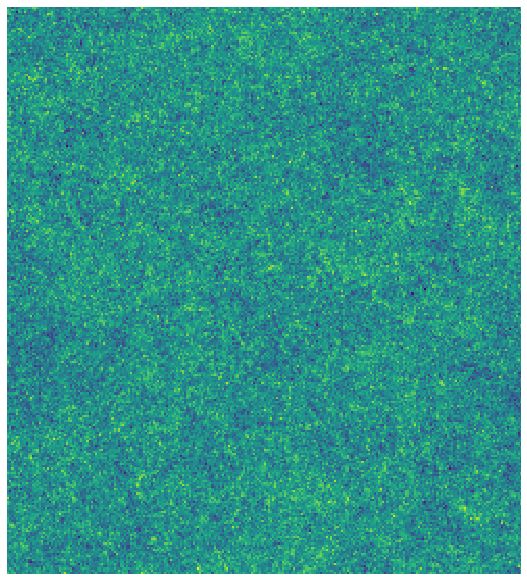
\includegraphics[scale=.38]{Results/GaussianRandomFieldSize400Alpha1.pdf}}
\hspace{8mm}
\subfloat[$\alpha = 3$]{\label{fig:GaussianRandomFieldSize400Alpha3.pdf}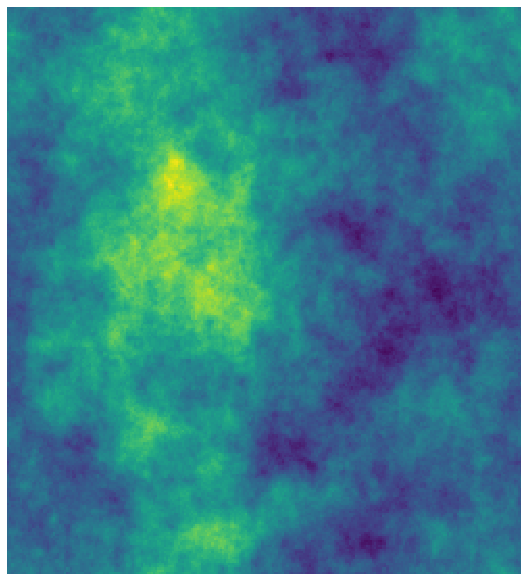
\includegraphics[scale=.38]{Results/GaussianRandomFieldSize400Alpha3.pdf}}
\hspace{8mm}
\subfloat[$\alpha = 5$]{\label{fig:GaussianRandomFieldSize400Alpha5.pdf}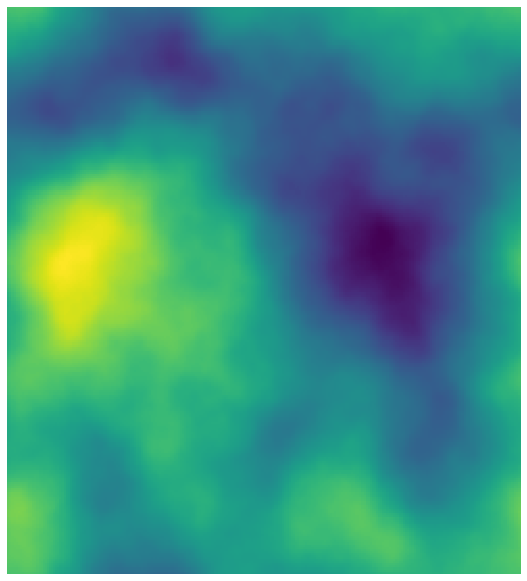
\includegraphics[scale=.38]{Results/GaussianRandomFieldSize400Alpha5.pdf}}
\caption{Gaussian Random Fields for various $\alpha$'s}
\label{fig:GaussianRandomField}
\end{figure}

Just as there is spatial autocorrelation, there is temporal autocorrelation, when the values of the field over the entire time period do not change
drastically. In principle, there can be different levels of autocorrelation over time and over space. However, for simplicity, in our analyses we will
use the same level of autocorrelation in all directions, determined by parameter~$\alpha$.

\subsection{Measures of Autocorrelation}
\label{sec:Materials and Methods/Measures of Autocorrelation}

In the geosciences, there are additional measures of spatial autocorrelation \cite{Eshel2011, Storch1999}. One frequently used is Moran's $I$~\cite{Moran1950, Hubert1981, PySAL}. Figure~\ref{fig:plotMoransIAndBeta} shows the relationship between Moran's $I$, using a uniform kernel with a bandwidth equal to~$10$, and the $\alpha$ of our simulated GRF's.

One can also devise an autocorrelation measure from the singular values of a dataset. Each singular value indicates the amount of variance explained by its associated mode. For fields with autocorrelation, the sorted list of singular values decays quickly. A power law can be fitted to this list, with an exponent which we call $\beta$.

A high $\alpha$ implies a high Moran's $I$ and a high $\beta$, which, in turn, implies some singular values are close to zero. Therefore, spatial fields with high levels of autocorrelation are described by matrices which are approximate rank deficient. This allows for data reduction without losing much information.

\begin{figure}[H]
\centering
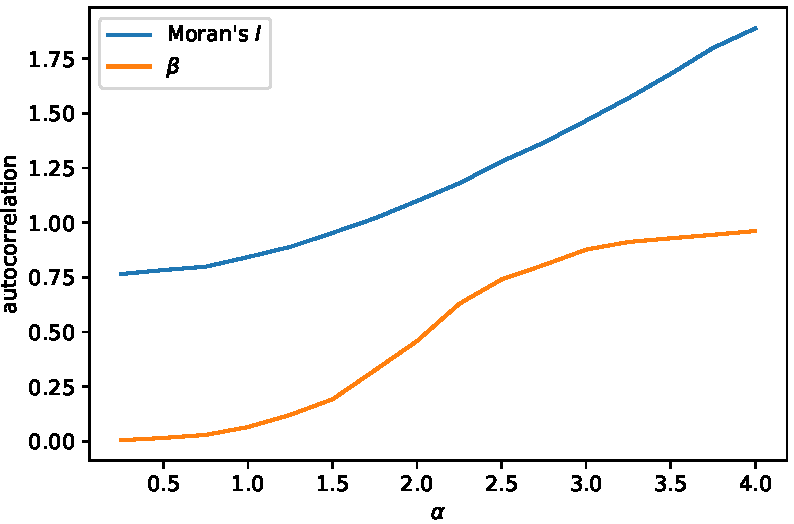
\includegraphics[width=80mm]{Results/plotMoransIAndBeta.pdf}
\caption[Various measures of autocorrelation]{Measures of autocorrelation as a function of $\alpha$}
\label{fig:plotMoransIAndBeta}
\end{figure}

\section{Results}
\label{sec:Results}

There are several SVD implementations that can be used to analyse large datasets efficiently by exploiting autocorrelation and rank deficiency.
Additional methods exist, though the ones covered here have three main benefits: coarsening is an easy-to-implement method, randomised dimensionality
reduction provides the best possible approximation for any level of reduction and the QR decomposition provides an exact and efficient result when
interested in the SVD of the product of two matrices.

To help researchers identify situations where different SVD approaches are beneficial, we have constructed the decision tree in figure~\ref{fig:FlowDiagram}. The first question to be answered is whether the SVD will be applied to a single matrix or to the product of two matrices. For single fields, the data may be small enough to fit in the memory of a computer. Then, a regular SVD is the best option. If the dataset is too large, two alternatives exists which provide an approximate answer: coarsening and randomised dimensionality reduction. These will be discussed in section~\ref{sec:Results/SVD of a Single Matrix}.

\begin{figure}[H]
\centering
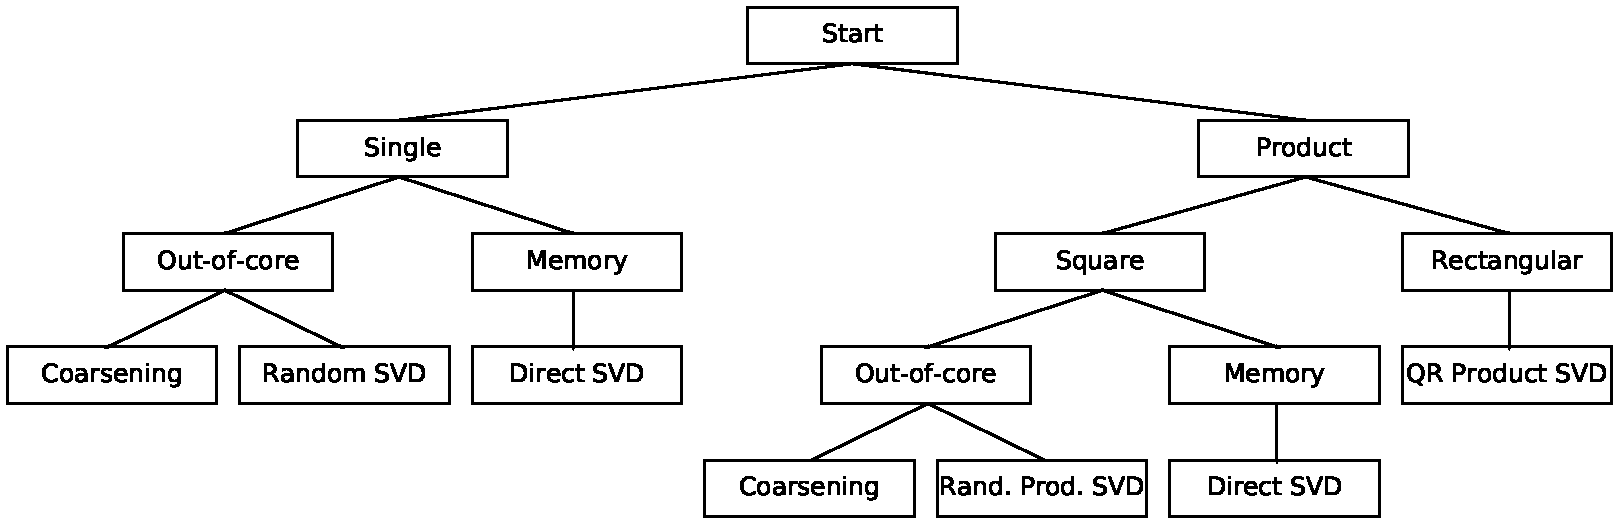
\includegraphics[width=\textwidth]{Results/FlowDiagram.pdf}
\caption{Decision tree describing the possible SVD techniques}
\label{fig:FlowDiagram}
\end{figure}

When the SVD is performed on the product of two matrices, the best course of action depends on whether the matrices are square or rectangular. The rank of a matrix is at most the size of the smallest side, which, for rectangular matrices, can be small. How to exploit this fact is described in section~\ref{sec:Results/Product SVD of Rectangular Matrices}. Square matrices small enough to fit in memory can be analysed directly. Variations of coarsening and dimensionality reduction can assist analyses of larger datasets, discussed in section~\ref{sec:Results/Product SVD of Square Matrices}.

Using simulated spatio-temporal fields with different levels of autocorrelation, we first study the relation between data characteristics and the
accuracy of different SVD implementations. Then, the lessons learned are verified using real-world datasets. We discuss which type of problems could
be tackled with which SVD implementation and predict the error incurred by using approximations based on the level of autocorrelation of the input
data.

\subsection{SVD of a Single Matrix} % Consider moving case studies to the end. RZ and RG prefer this, LB does not.
\label{sec:Results/SVD of a Single Matrix}

\subsubsection{Approximate SVD of a Single Matrix via Coarsening}
\label{sec:Results/Approximate SVD of a Single Matrix via Coarsening}

When a spatial field has large scale structure, the values of neighbouring cells do not change drastically. Perhaps these cells can be aggregated together to produce a smaller dataset which still faithfully describes the original field. Here, we exploit the data redundancy described in section~\ref{sec:Materials and Methods} and coarsen two dimensional GRF's.

Figure~\ref{fig:plotSingleSpatialFieldViaCoarsening} shows the error in a coarsening process for matrices of various~$\alpha$'s and for different coarsening window sizes. The error is determined as the norm of the difference between the original matrix and the coarsened version, divided by the norm of the original~\cite{Bogaardt2018}. Other measures of similarity, such as the correlation between the two datasets, are likely to show the same effects. % RZ: remove.this statement will puzzle the reviewers and prompt them to ask questions ... LB: I prefer keeping this in, but changed the emphasis a bit.
Note that coarsening a two dimensional field at level 5 reduces the dataset by $25$ times. For fields with high autocorrelation, e.g. $\alpha=3$, the coarsened version differs by less than~$10\%$ from the original.

\begin{figure}[H]
\centering
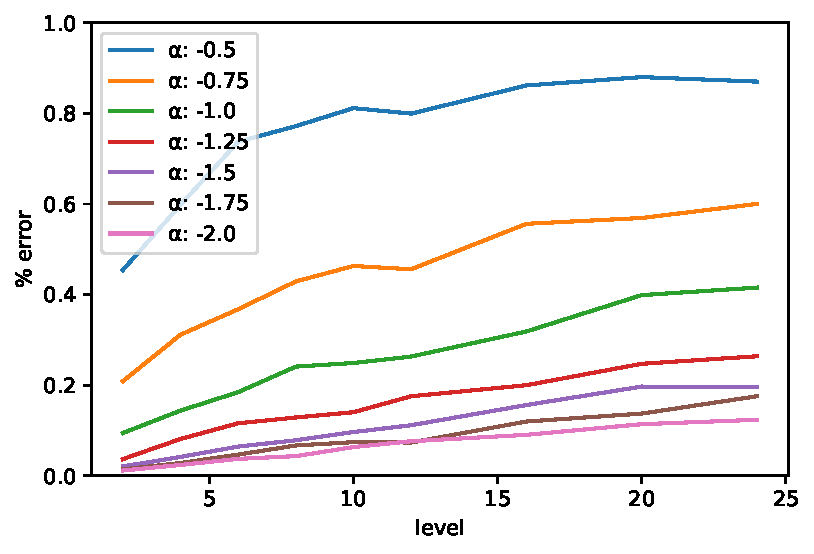
\includegraphics[width=80mm]{Results/plotSingleSpatialFieldViaCoarsening.pdf}
\caption[Error after coarsening]{Error in the SVD of a coarsened spatial field for various $\alpha$'s and Moran's $I$'s}
\label{fig:plotSingleSpatialFieldViaCoarsening}
\end{figure}

\subsubsection{Approximate SVD of a Single Matrix via Dimensionality Reduction}
\label{sec:Results/Approximate SVD of a Single Matrix via Dimensionality Reduction}

An alternative method of reducing the size of a matrix is via randomised dimensionality reduction. During dimensionality reduction, the number of basis-vectors of a matrix is truncated to the~$l$ most important ones, similar to finding an $\epsilon$-rank approximation. Remember from section~\ref{sec:Materials and Methods} that, if a dataset is noisy, low rank approximations can contain most of the relevant information. Furthermore, matrices with low rank require less storage space and fewer flops for vector multiplications.

A random algorithm exists which performs an approximate rank decomposition of a large matrix efficiently. The mathematics behind this algorithm is reviewed extensively elsewhere, here we examine its performance on datasets with autocorrelation~\cite{Halko2011, Li2016}. The main idea is to sample from the original values, taking as many values as needed to achieve the required accuracy. One of its benefits is that this algorithm requires only a small number of passes over the data, which, for large matrices stored out-of-core, reduces reading time. Additionally, the incurred error in the approximation can be made arbitrarily small by adjusting~$l$ and~$\epsilon$, giving the researcher full control over the balance between computation cost and accuracy.

Figure~\ref{fig:reduceSizeRandomisedSquare} depicts the calculation in this process, which first reduces the input matrix to a smaller square matrix of $l$~by~$l$. It also provides two projection matrices which rotate the rows and columns of this smaller matrix back as close as possible to the bases of the original input. Subsequently, the SVD is applied to the small $l$~by~$l$ matrix, which results in a fast and efficient approximation of the matrix's decomposition with an error of the order of the size of the largest truncated singular value~\cite{Martinsson2016, Halko2011}.

\begin{figure}[H]
\centering
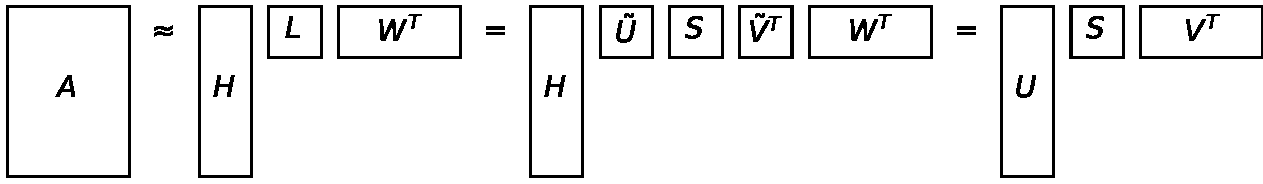
\includegraphics[width=100mm]{Results/reduceSizeRandomisedSquare.pdf}
\caption[Approximate randomised SVD]{Visualising the calculation of an approximate SVD via dimensionality reduction}
\label{fig:reduceSizeRandomisedSquare}
\end{figure}

The calculations in the \textit{Jupyter Notebook}, which is provided in the suplementary material, show that the errors induced by the randomised SVD procedure are very small, even for high levels of reduction~\cite{Bogaardt2018}. This is especially true for fields with autocorrelation. Looking at figure~\ref{fig:plotMoransIAndBeta}, this is not surprising; high autocorrelation means a high $\beta$ which implies that the singular values decay quickly and that the last modes contribute little information to the dataset.

This randomised technique achieves much lower errors than coarsening. The coarsening procedure has several advantages though. For one, it is intuitive and the results are easy to interpret. It is also trivial to implement. Additionally, different coarsening levels can be applied to different directions. This is especially advantages when directions have different levels of autocorrelation or are recorded at different resolutions. Finally, the predictions of figure~\ref{fig:plotSingleSpatialFieldViaCoarsening} can help researchers determine at what resolution to gather their data in the first place. In domains were satellite data is used, datasets are often not very detailed because the imaging resolution is low. Unlike local analyses of developed countries, where high resolution data is becoming more accessible, for continental or global analyses, coarse spatial resolution data may simply be the only option.

\subsubsection{Case Study of an SVD of a Single Matrix}
\label{sec:Results/Case Study of an SVD of a Single Matrix} % Our ERA5 data runs from 1 April 2012 to 10 April 2012: ten days every 6 hours.

Coarsening and dimensionality reduction are particularly useful for spatial fields with high levels of autocorrelation. As an example of this, we examine humidity and cloud cover data from the ERA5 datasets for a single time period measured on 1 April 2012. ERA5 is an atmospheric reanalysis of the global climate using high spatial resolution forecasts, produced by combining models with observations~\cite{Dee2011}. It contains estimates of atmospheric parameters such as air temperature, pressure and wind at different altitudes.

Clearly, the ERA5 humidity and cloud cover fields are not GRF's. Nonetheless, we can get an idea of the accuracy of an SVD after data reduction if we estimate the levels of autocorrelation. This can verify whether simulated GRF's are reasonable representations of real-world datasets. The humidity field has a Moran's $I \approx 0.98$, while the cloud cover data shows less structure with a Moran's $I \approx 0.82$. The estimations for~$\alpha$ were unreliable as the power law did not fit properly, though figure~\ref{fig:plotMoransIAndBeta} can help us translate the measures and suggests the fields are equivalent to GRF's with an $\alpha \sim 3.5$ and $\alpha \sim 2.5$, respectively.

The coarsening predictions of figure~\ref{fig:plotSingleSpatialFieldViaCoarsening} indicate the first field is expected to incur errors around a few percent for size reductions between~$2$ and~$8$, while for the second field we should see errors between~$5\%$ and~$15\%$. The calculations in the \textit{Jupyter Notebook} in the supplementary material show that this prediction is fairly accurate, perhaps slightly pessimistic. The humidity field, which has the largest autocorrelation, only incurred an error of $1\%$ when halved in size. For the cloud cover data, this values was closer to $4\%$. Likewise, we can apply the randomised dimensionality reduction technique to the fields. As expected, this resulted in very small errors, below $1\%$. If a researcher cares most about accuracy, dimensionality reduction is the best option.

\subsection{Product SVD of Rectangular Matrices}
\label{sec:Results/Product SVD of Rectangular Matrices}

In real-world applications, researchers often wants to find the relation between two fields. Analyses such as the MCA and CCA, discussed in section~\ref{sec:Introduction}, expose patterns in the data which occur frequently and simultaneously~\cite{Eshel2011, Storch1999}. In some domains, the term SVD is used synonymously with MCA. If the input datasets have the various spatial gridpoints as rows and the sample of recorded values over time as columns, multiplying them gives their cross-covariance matrix. An SVD of this cross-covariance matrix provides the row- and the column vectors which covary maximally~\cite{Bretherton1992}. Multiplying the two spatio-temporal fields, however, can result in a rather large matrix which may not fit in \textit{RAM}-memory and would be difficult to analyse. This section and section~\ref{sec:Results/Product SVD of Square Matrices} describe possible solutions.

\subsubsection{Exact Product SVD of Rectangular Matrices via QR Decomposition}
\label{sec:Results/Exact Product SVD of Rectangular Matrices via QR Decomposition} % If we rephrase the article to place more emphasis on the out-of-coire problem, then explain here why the large intermediate matrix is a problem.

For highly rectangular datasets, when there are many spatial gridpoints but few temporal samples, the resulting cross-covariance matrix is obviously rank deficient. Performing a rank decomposition on each dataset before multiplying them allows the SVD to be calculated in an efficient manner~\cite{Chan1982, Tygert2017}. Figure~\ref{fig:qrProductSVD} depicts the calculation in this technique. Using the QR decomposition, the input datasets are first transformed into two small, square matrices together with rectangular orthonormal basis vectors. The SVD is then performed on the product of the square matrices, giving a mathematically identical result to the full SVD while never forming an unnecessarily large, intermediate matrix.

\begin{figure}[H]
\centering
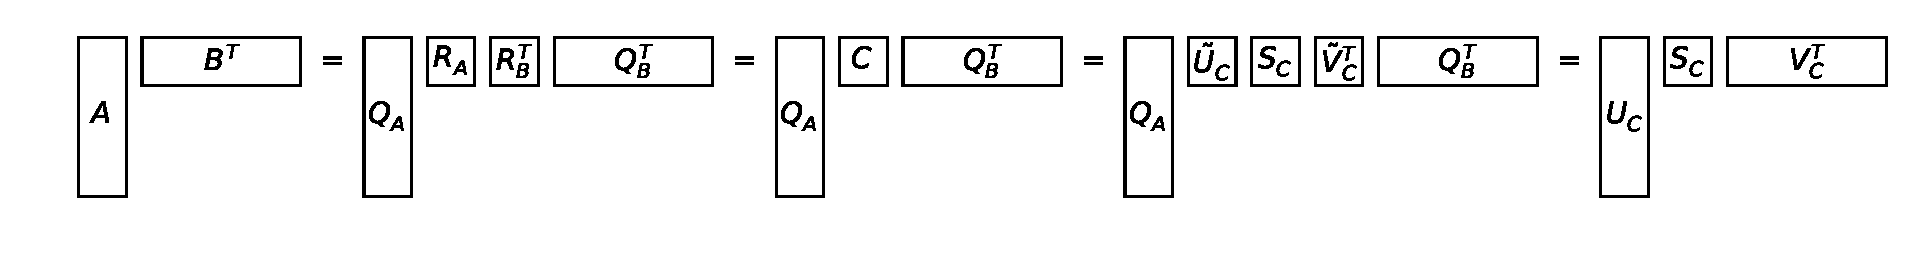
\includegraphics[width=\textwidth]{Results/qrProductSVD.pdf}
\caption[Exact SVD via QR decomposition]{Visualising the calculation of the exact SVD of a product via QR decomposition}
\label{fig:qrProductSVD}
\end{figure}

\subsubsection{Case Study of a Product SVD of Rectangular Matrices}
\label{sec:Results/Case Study of a Product SVD of Rectangular Matrices}

Let's apply the QR decomposition technique to phenological datasets. Phenology is the science that studies recurring biological events such as leafing and blooming as well as their causes and variations in space and time. Spatio-temporal fields of remotely sensed images can be used to derive various phenological metrics. One important family of such metrics are the \textit{Extended Spring Indices} (SI-x), which are based on a suite of models that transform daily temperatures into consistent phenological metrics~\cite{Schwartz2013}. In particular, we take versions of the Leaf and the Bloom index, depicted in Figure~\ref{fig:phenologydata}, which were recently generated for the US by adapting the SI-x models to a cloud computing environment~\cite{Izquierdo2015}. 

\begin{figure}[H]
\centering
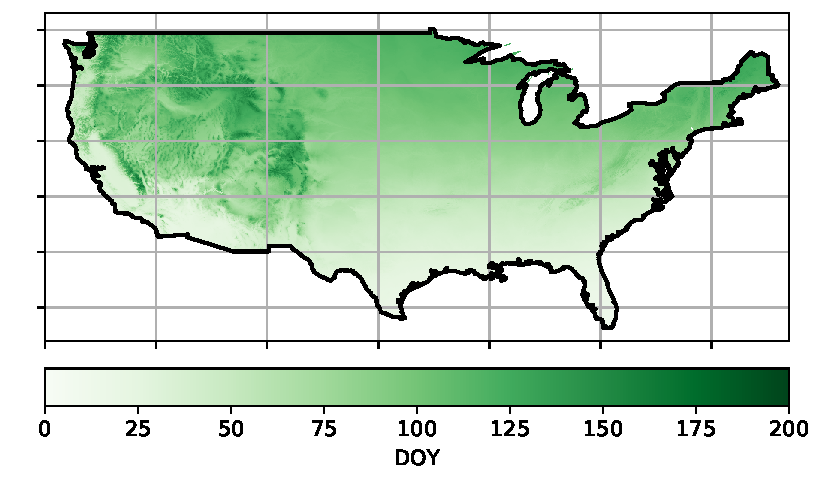
\includegraphics[width=7.5cm]{Results/Leafmean.pdf} ~~~~~ 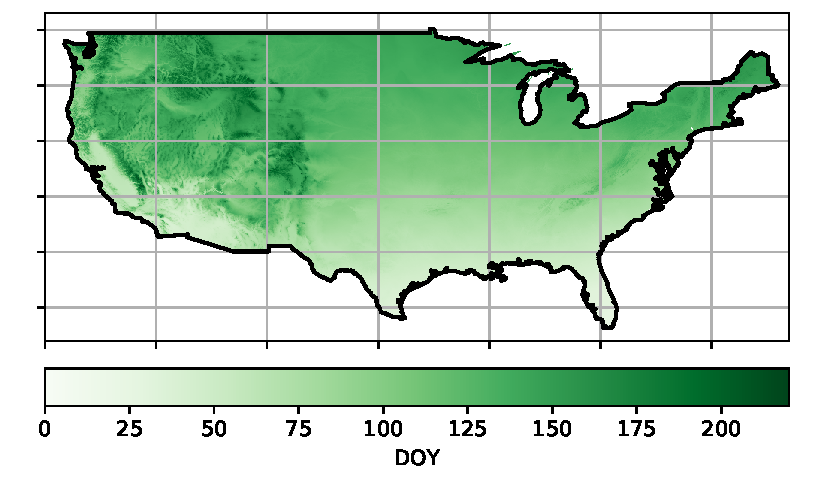
\includegraphics[width=7.5cm]{Results/Bloommean.pdf}
\caption{Average of phenology products: Leaf [l] and Bloom [r] from $1989$ to $2014$}
\label{fig:phenologydata}
\end{figure}

Both datasets span from $1989$ to $2014$ and have a $1\text{km}$ spatial resolution, meaning there are far fewer time periods than spatial gridpoints, giving highly rectangular matrices. In fact, each dataset contains $30$ million rows and $26$ columns and is about $3.1$ GB large. Their cross-covariance would be $30$ million rows by $30$ million columns and about $3.6$ PB in size. Luckily, this product matrix need not be created; the SVD is performed on a $26$ rows by $26$ columns matrix, stored in memory.

For the SVD via QR decomposition, the level of autocorrelation is irrelevant because this technique provides a mathematically exact result. Indeed, the \textit{Jupyter Notebook} in the supplementary material, as well as work being prepared for publication, shows that this technique provides the full SVD of the cross-covariance matrix for these datasets in a matter of seconds, without ever exceeding the \textit{RAM}-memory~\cite{Bogaardt2018, ZuritaMilla2018}. The first mode for both Leaf and Bloom data can be mapped back into the original geographical shape, as depicted in Figure~\ref{fig:maps}.

\begin{figure}[H]
\centering
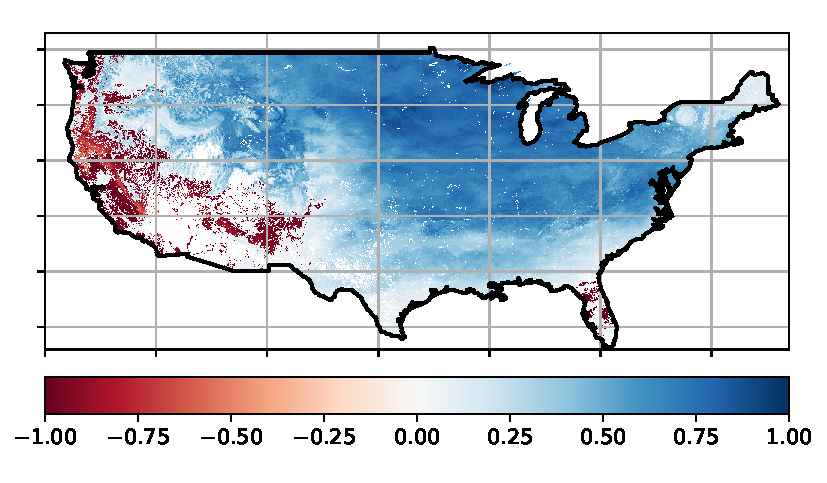
\includegraphics[width=7.5cm]{Results/SpatialModeV01Grid.pdf} ~~~~~ 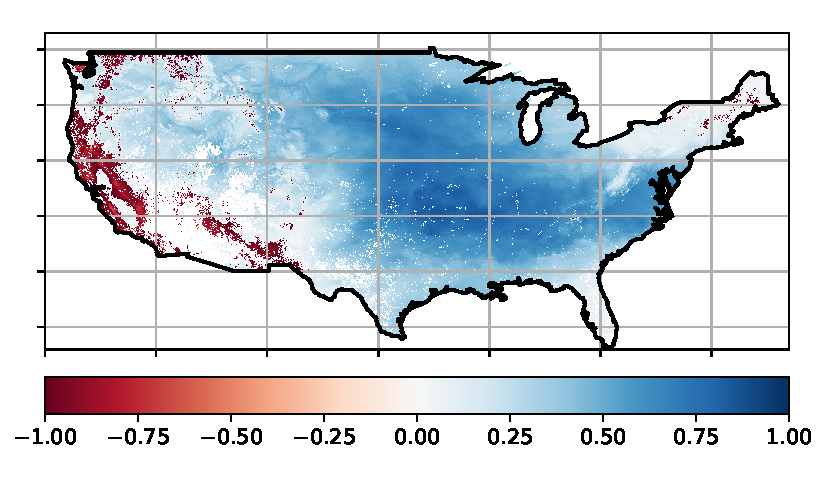
\includegraphics[width=7.5cm]{Results/SpatialModeU01Grid.pdf}
\caption{Phenology products: Leaf [l] and Bloom [r] data projected onto the first principal component}
\label{fig:maps}
\end{figure}

\subsection{Product SVD of Square Matrices}
\label{sec:Results/Product SVD of Square Matrices}

\subsubsection{Approximate Product SVD of Square Matrices via Coarsening}
\label{sec:Results/Approximate Product SVD of Square Matrices via Coarsening}

In section~\ref{sec:Results/Approximate SVD of a Single Matrix via Coarsening}, we saw coarsening can reduce the size of a single spatial field. We can also coarsen two spatio-temporal fields before analysing their cross-covariance matrix. Figure~\ref{fig:plotProductSpatialTemporalFieldsViaCoarsening} shows the percentage error for various simulated spatio-temporal fields. Note that only the spatial directions are coarsened in our calculation. This is because the time direction gets consumed in the matrix product of the MCA or CCA and coarsening it will not decrease the size of the cross-covariance matrix nor speed up the SVD. While coarsening two spatial directions means each field is reduced by the square of the coarsening level, the cross-covariance matrix is reduced by this level to the power~$4$. As a result, the typical error in this product is larger than for the single field, though the speed up is also substantial. Clearly, the level of autocorrelation plays an important part, with larger~$\alpha$'s leading to less error.% Preliminary work shows the amount of error also depends on the similarity between the two spatio-temporal fields, though we leave deeper investigation of this aspect for further research. 

\begin{figure}[H]
\centering
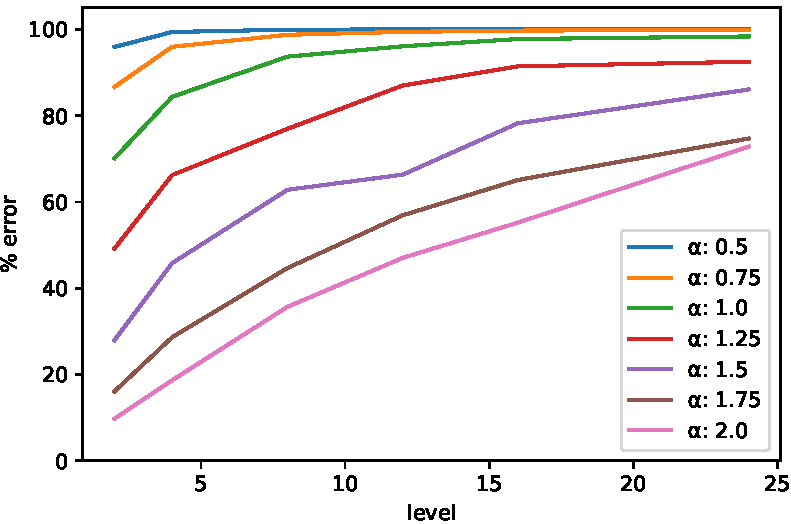
\includegraphics[width=80mm]{Results/plotProductSpatialTemporalFieldsViaCoarsening.pdf}
\caption[Error after coarsening]{Error in the SVD of the product of two coarsened fields for various $\alpha$'s}
\label{fig:plotProductSpatialTemporalFieldsViaCoarsening}
\end{figure}

\subsubsection{Approximate Product SVD of Square Matrices via Dimensionality Reduction}
\label{sec:Results/Approximate Product SVD of Square Matrices via Dimensionality Reduction}

%\enlargethispage{6mm} % Remember
The randomised dimensionality reduction process may also speed up the SVD analysis of two spatio-temporal fields. The reduction can be applied to each of the fields before they are multiplied into the cross-covariance matrix. Similar to the QR decomposition of section~\ref{sec:Results/Exact Product SVD of Rectangular Matrices via QR Decomposition}, it has the advantage that the SVD is performed on a small $l$~by~$l$ matrix. This calculation is visualised in figure~\ref{fig:randomisedSquareProductSVD}. In the first step, the input datasets are decomposed using the algorithm discussed in section~\ref{sec:Results/Approximate SVD of a Single Matrix via Dimensionality Reduction} and reviewed extensively elsewhere~\cite{Halko2011, Li2016}. Again, the main idea behind the algorithm is to sample from the original values, taking as many values as needed to achieve the required accuracy. Subsequently, the inner matrices are multiplied and the SVD is performed on the resulting, small matrix.

\begin{figure}[H]
\centering
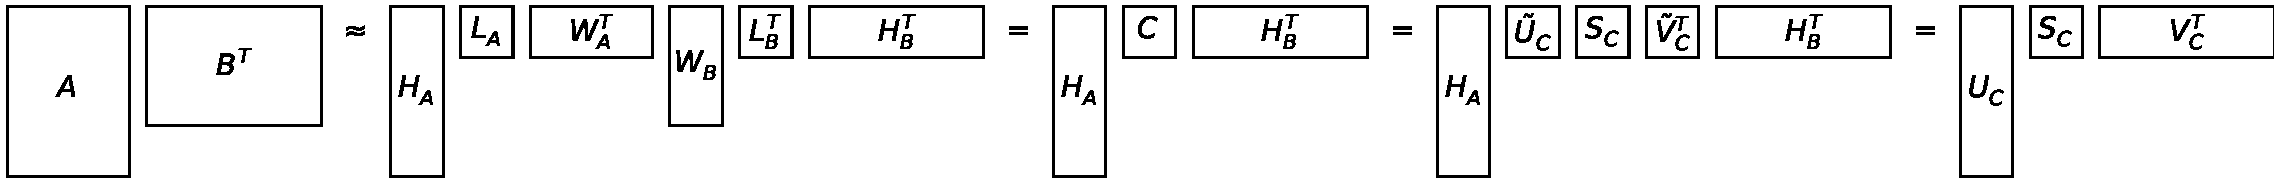
\includegraphics[width=\textwidth]{Results/randomisedSquareProductSVD.pdf}
\caption[Approximate product SVD]{Visualising the calculation of an approximate SVD for the product of two fields using dimensionality reduction}
\label{fig:randomisedSquareProductSVD}
\end{figure}

After generating various GRF's, the reduced cross-covariance matrix is compared with the original. Figure~\ref{fig:plotRandomisedSizeReducedMatrixProduct} shows that the results are not satisfactory for fields with a small $\alpha$, but high levels of autocorrelation allow for substantial savings in computation time without incurring much error. Note that, when performing an MCA or CCA on a spatio-temporal field, the spatial directions are flattened and some of the spatial autocorrelation is lost. This partially explains why the error is substantial for low $\alpha$.

The reduction of the number of dimensions of each input dataset before an MCA or CCA is actually advised by some researchers, as a method to filter out noise~\cite{Barnett1987}. Especially when the number of temporal samples is small, outliers and random fluctuations could affect the result~\cite{Bretherton1992}. This is because any statistical analysis will choose its regression-coefficients so as to optimize the fit. It may occur that two noise-vectors in the two fields coincidentally covary and show up as dominant modes. Prefiltering can alleviate this risk.

\begin{figure}[H]
\centering
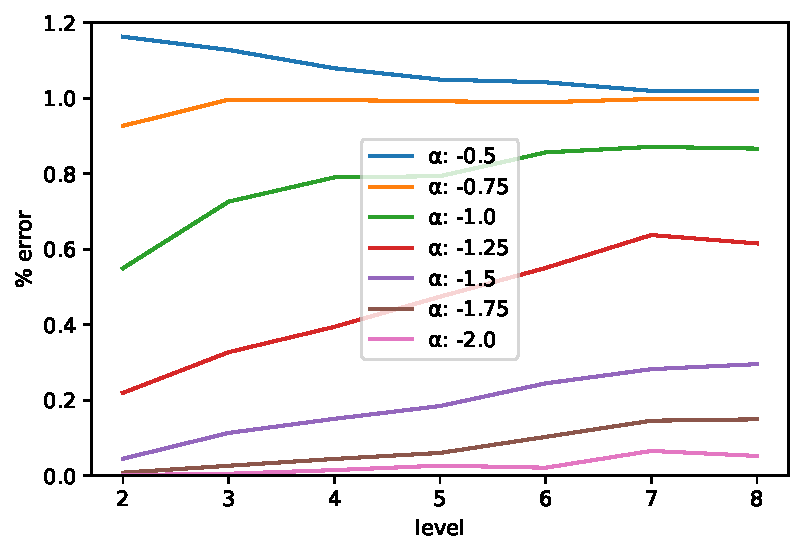
\includegraphics[width=80mm]{Results/plotRandomisedSizeReducedMatrixProduct.pdf}
\caption[Error after reduction]{Error in the SVD of the product of two reduced fields for various $\alpha$'s}
\label{fig:plotRandomisedSizeReducedMatrixProduct}
\end{figure}

\subsubsection{Case Study of a Product SVD of Square Matrices}
\label{sec:Results/Case Study of a Product SVD of Square Matrices}

The JRA55 data is an atmosphere reanalysis product which includes quantities such as humidity, pressure and temperature~\cite{Kobayashi2015}. Recently, these quantities were used to determine the total meridional energy transport and latent heat, measures important to understand the global climate~\cite{Liu2018}. As an example of our reduction techniques for matrix products, we are using a Mercator projection of the energy transport and latent heat, recorded monthly from 1979 to 2015. Although the spatially flattened matrices are not completely square, their high resolution in the time direction make them substantially less rectangular than the phenology data from section~\ref{sec:Results/Case Study of a Product SVD of Rectangular Matrices}. Therefore, this serves as a good use case for the coarsening and dimensionality reduction techniques for a square product SVD.

The energy field has a Moran's $I \approx 0.93$, while the latent heat field has a Moran's $I \approx 0.86$. The estimations for~$\alpha$ were unreliable, though figure~\ref{fig:plotMoransIAndBeta} can help us translate the measures and suggests the fields are equivalent to GRF's with an $\alpha \sim 3.0$ and $\alpha \sim 2.5$, respectively. The analyses of section~\ref{sec:Results/Approximate Product SVD of Square Matrices via Coarsening} and of section~\ref{sec:Results/Approximate Product SVD of Square Matrices via Dimensionality Reduction} make the prediction that, for such~$\alpha$ levels, our data reduction techniques result in errors which are quite high. In contrast, we found that coarsening the fields before applying an SVD on their product merely resulted in an error of $8\%$ when the data was halved and an error around $16\%$ when the data was reduced by a factor of $4$. For the dimensionality reduction technique, as well, the predictions overstated the observed error, which were around a few percent, even for high levels of size reduction.

%%%%%%%%%%%%%%%%%%%%%%%%%%%%%%%%%%%%%%%%%%
%\subsection{Subsection}

%\subsubsection{Subsubsection}

%Bulleted lists look like this:
%\begin{itemize}[leftmargin=*,labelsep=5.8mm]
%\item	First bullet
%\item	Second bullet
%\item	Third bullet
%\end{itemize}

%Numbered lists can be added as follows:
%\begin{enumerate}[leftmargin=*,labelsep=4.9mm]
%\item	First item 
%\item	Second item
%\item	Third item
%\end{enumerate}

%The text continues here.

%\subsection{Figures, Tables and Schemes}

%All figures and tables should be cited in the main text as Figure 1, Table 1, etc.

%\begin{figure}[H]
%\centering
%
\includegraphics[width=2 cm]{Definitions/logo-mdpi}
%\caption{This is a figure, Schemes follow the same formatting. If there are multiple panels, they should be listed as: (\textbf{a}) Description of what is contained in the first panel. (\textbf{b}) Description of what is contained in the second panel. Figures should be placed in the main text near to the first time they are cited. A caption on a single line should be centered.}
%\end{figure} 

%\begin{table}[H]
%\caption{This is a table caption. Tables should be placed in the main text near to the first time they are cited.}
%\centering
%% \tablesize{} %% You can specify the fontsize here, e.g. \tablesize{\footnotesize}. If commented out \small will be used.
%\begin{tabular}{ccc}
%\toprule
%\textbf{Title 1}	& \textbf{Title 2}	& \textbf{Title 3}\\
%\midrule
%entry 1		& data			& data\\
%entry 2		& data			& data\\
%\bottomrule
%\end{tabular}
%\end{table}

%\subsection{Formatting of Mathematical Components}

%This is an example of an equation:

%\begin{equation}
%a + b = c
%\end{equation}
%% If the documentclass option "submit" is chosen, please insert a blank line before and after any math environment (equation and eqnarray environments). This ensures correct linenumbering. The blank line should be removed when the documentclass option is changed to "accept" because the text following an equation should not be a new paragraph. 

%Please punctuate equations as regular text. Theorem-type environments (including propositions, lemmas, corollaries etc.) can be formatted as follows:
%% Example of a theorem:
%\begin{Theorem}
%Example text of a theorem.
%\end{Theorem}

%The text continues here. Proofs must be formatted as follows:

%% Example of a proof:
%\begin{proof}[Proof of Theorem 1]
%Text of the proof. Note that the phrase `of Theorem 1' is optional if it is clear which theorem is being referred to.
%\end{proof}
%The text continues here.

%%%%%%%%%%%%%%%%%%%%%%%%%%%%%%%%%%%%%%%%%%
\section{Discussion}
\label{sec:Discussion}
%Authors should discuss the results and how they can be interpreted in perspective of previous studies and of the working hypotheses. The findings and their implications should be discussed in the broadest context possible. Future research directions may also be highlighted.

\subsection{Further Work and Caveats}
\label{sec:Discussion/Further Work}

Much of the analysis here relies on knowledge of the level of autocorrelation, which may be difficult to determine for large datasets. The \textit{Jupyter Notebook} accompanying this article includes an algorithm which estimates Moran's $I$ based on a sample of gridpoints. This speeds up the calculation substantially compared with the full calculation and gives very similar results. A spin-off from the current article could be to further develop this approximate measure of Moran's $I$. Additional areas of future research include relaxing the assumption that the autocorrelation in the time direction is similar to that in the spatial directions. In fact, it is more realistic to allow for different levels of autocorrelation in all directions and to have a version of Moran's $I$ which can estimate these values.

Furthermore, a warning about autocorrelation and standardisation. In MCA's, the time series of each spatial gridpoint is centred about its mean and in CCA's, each gridpoint is standardised. These operations destroy much of the spatial autocorrelation, as it can affect neighbouring cells differently. When researcher choose the coarsening technique, this should occur before any additional data processing steps.

Unlike the coarsening procedure, the dimensionality reduction is not applied on each spatial field for each time period, but rather on the entire spatially flattened time series. Therefore, the level of spatial autocorrelation may not be as important as the level of temporal autocorrelation. Further work can examine how to apply the reduction to the spatial part of the spatio-temporal fields, before it is flattened. Alternative solutions, which retain the spatial structure, may include 3D tensor operations such as \textit{Higher-Order Singular Value Decomposition} (HOSVD)~\cite{Tucker1964}.

\subsection{Conclusion}
\label{sec:Discussion/Summary} % If we change the emphasis to out-of-core, change this conclusion to say all techniques work on data which is too larg for internal memory, but randomised dimensionaliy reduction works best in terms of accuracy.

Randomised dimensionality reduction works best for geo-datasets which are too large for internal memory. It requires only a small number of passes over the data, which decreases storage reading time. It also allows the researcher to balance computation cost with accuracy, by tuning the algorithm's parameters. Performing analyses at a coarse level can be beneficial when data collection is difficult and provides an intuitive and easy-to-implement alternative. These techniques require at least some autocorrelation in the fields, which results in approximate rank deficient datasets. In general, rank decompositions can speed up calculations by splitting datasets into smaller matrices of full rank. For the product of rectangular matrices, this can even give a mathematically exact result.
\\ % Remember

%%%%%%%%%%%%%%%%%%%%%%%%%%%%%%%%%%%%%%%%%%
%\section{Conclusions}

%This section is not mandatory, but can be added to the manuscript if the discussion is unusually long or complex.

%%%%%%%%%%%%%%%%%%%%%%%%%%%%%%%%%%%%%%%%%%
%\section{Patents}
%This section is not mandatory, but may be added if there are patents resulting from the work reported in this manuscript.

%%%%%%%%%%%%%%%%%%%%%%%%%%%%%%%%%%%%%%%%%%
\vspace{6pt} 

%%%%%%%%%%%%%%%%%%%%%%%%%%%%%%%%%%%%%%%%%%
%% optional
%\supplementary{The following are available online at \linksupplementary{s1}, Figure S1: title, Table S1: title, Video S1: title.}

% Only for the journal Methods and Protocols:
% If you wish to submit a video article, please do so with any other supplementary material.
% \supplementary{The following are available at \linksupplementary, Figure S1: title, Table S1: title, Video S1: title. A supporting video article is available at doi: link.}

%%%%%%%%%%%%%%%%%%%%%%%%%%%%%%%%%%%%%%%%%%
\authorcontributions{Conceptualization, R.Z.M.; Methodology, L.B.; Software, L.B.; Validation, R.G., R.Z.M. and E.I.V.; Formal Analysis, L.B.; Investigation, L.B.; Resources, R.G., R.Z.M. and E.I.V.; Data Curation, R.G., R.Z.M. and E.I.V.; Writing—Original Draft Preparation, L.B.; Writing—Review \& Editing, R.G., R.Z.M. and E.I.V.; Visualization, L.B.; Supervision, R.G. and R.Z.M.; Project Administration, R.G.; Funding Acquisition, R.Z.M.}

%%%%%%%%%%%%%%%%%%%%%%%%%%%%%%%%%%%%%%%%%%
\funding{This research was funded by the Nederlandse Organisatie voor Wetenschappelijk Onderzoek (NWO).}

%%%%%%%%%%%%%%%%%%%%%%%%%%%%%%%%%%%%%%%%%%
%\acknowledgments{In this section you can acknowledge any support given which is not covered by the author contribution or funding sections. This may include administrative and technical support, or donations in kind (e.g. materials used for experiments).}

%%%%%%%%%%%%%%%%%%%%%%%%%%%%%%%%%%%%%%%%%%
\conflictsofinterest{The authors declare no conflict of interest. The founding sponsors had no role in the design of the study; in the collection, analyses, or interpretation of data; in the writing of the manuscript, and in the decision to publish the results.} 

%%%%%%%%%%%%%%%%%%%%%%%%%%%%%%%%%%%%%%%%%%
%% optional
\abbreviations{The following abbreviations are used in this manuscript:\\

\noindent 
\begin{tabular}{@{}ll}
SVD & Singular value decomposition\\
PLS & Partial least squares\\
MCA & Maximum covariance analysis\\
CCA & Canonical correlation analysis\\
MNF & Minimum noise fraction\\
PC & Principle component\\
EOF & Empirical orthogonal function\\
GRF & Gaussian random field\\
SI-x & Extended spring indices\\
ERA5 & European fifth generation reanalysis\\
JRA55 & Japanese 55-year reanalysis\\
HOSVD & Higher-order singular value decomposition
\end{tabular}}

%%%%%%%%%%%%%%%%%%%%%%%%%%%%%%%%%%%%%%%%%%
%% optional
%\appendixtitles{no} %Leave argument "no" if all appendix headings stay EMPTY (then no dot is printed after "Appendix A"). If the appendix sections contain a heading then change the argument to "yes".
%\appendixsections{multiple} %Leave argument "multiple" if there are multiple sections. Then a counter is printed ("Appendix A"). If there is only one appendix section then change the argument to "one" and no counter is printed ("Appendix").
%\appendix
%\section{}
%\subsection{}
%The appendix is an optional section that can contain details and data supplemental to the main text. For example, explanations of experimental details that would disrupt the flow of the main text, but nonetheless remain crucial to understanding and reproducing the research shown; figures of replicates for experiments of which representative data is shown in the main text can be added here if brief, or as Supplementary data. Mathematical proofs of results not central to the paper can be added as an appendix.

%\section{}
%All appendix sections must be cited in the main text. In the appendixes, Figures, Tables, etc. should be labeled starting with `A', e.g., Figure A1, Figure A2, etc. 

%%%%%%%%%%%%%%%%%%%%%%%%%%%%%%%%%%%%%%%%%%
% Citations and References in Supplementary files are permitted provided that they also appear in the reference list here. 

%=====================================
% References, variant A: internal bibliography
%=====================================
%\reftitle{References}
%\begin{thebibliography}{999}
% Reference 1
%\bibitem[Author1(year)]{ref-journal}
%Author1, T. The title of the cited article. {\em Journal Abbreviation} {\bf 2008}, {\em 10}, 142-149, DOI.
% Reference 2
%\bibitem[Author2(year)]{ref-book}
%Author2, L. The title of the cited contribution. In {\em The Book Title}; Editor1, F., Editor2, A., Eds.; Publishing House: City, Country, 2007; pp. 32-58, ISBN.
%\end{thebibliography}

% The following MDPI journals use author-date citation: Arts, Econometrics, Economies, Genealogy, Humanities, IJFS, JRFM, Laws, Religions, Risks, Social Sciences. For those journals, please follow the formatting guidelines on http://www.mdpi.com/authors/references
% To cite two works by the same author: \citeauthor{ref-journal-1a} (\citeyear{ref-journal-1a}, \citeyear{ref-journal-1b}). This produces: Whittaker (1967, 1975)
% To cite two works by the same author with specific pages: \citeauthor{ref-journal-3a} (\citeyear{ref-journal-3a}, p. 328; \citeyear{ref-journal-3b}, p.475). This produces: Wong (1999, p. 328; 2000, p. 475)

%=====================================
% References, variant B: external bibliography
%=====================================
\externalbibliography{yes}
\bibliography{Bibliography}

%%%%%%%%%%%%%%%%%%%%%%%%%%%%%%%%%%%%%%%%%%
%% optional
%\sampleavailability{Samples of the compounds ...... are available from the authors.}

%% for journal Sci
%\reviewreports{\\
%Reviewer 1 comments and authors’ response\\
%Reviewer 2 comments and authors’ response\\
%Reviewer 3 comments and authors’ response
%}

%%%%%%%%%%%%%%%%%%%%%%%%%%%%%%%%%%%%%%%%%%
\end{document}

